\section{Disagio psichico in medicina generale}

\subsection{Dimensione del problema}

Nella seconda metà del secolo scorso molti medici si sono resi conto del
grande peso del disagio psichico che riguardava la medicina generale.

Balint negli anni '50 aveva organizzato dei gruppi tra psichiatri e MMG
che si focalizzarono sulla relazione medico-paziente e su quanto questa
fosse importante, soprattutto nei pazienti con disagi psichici, come
azione terapeutica non farmacologica.

La stragrande maggioranza dei pazienti con disturbi psichiatrici viene
vista e trattata negli ambulatori dei MMG.

Secondo uno studio di Goldberg del 1992 i disturbi psichici in medicina
generale sono presenti in una misura variabile dal 25 al 35\%.

Negli anni 80-90 l'OMS, al fine di approfondire e quantificare il
problema emerso dai precedenti studi, ha affidato a Ustun e Sartorius il
compito di definire in termini epidemiologici il fenomeno su scala
internazionale.

Dagli studi emerse che le persone affette da disturbo psichico che si
rivolgevano al MMG erano il 10-25\% e solo una piccolissima parte
(1-2\%) accedeva alle cure specialistiche psichiatriche.

Poiché lo studio fu eseguito su scala internazionale e considerando che
la popolazione che accede alle cure primarie è la stragrande
maggioranza, i dati ottenuti potrebbero essere considerati come un dato
di reale prevalenza nella popolazione generale.

\begin{figure}[!ht]
\centering
	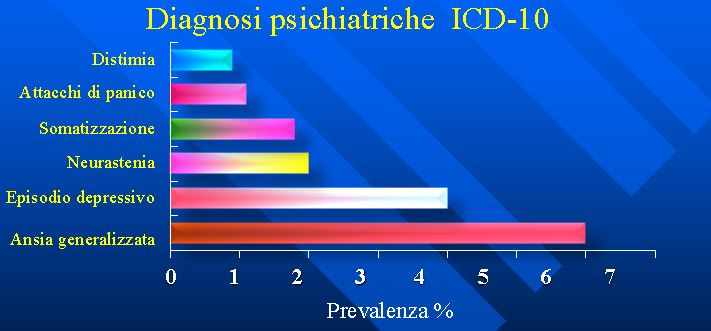
\includegraphics[width=0.8\textwidth]{42/image1.jpeg}
	\end{figure}
	
Secondo
vari studi svolti successivamente anche in Italia, a Bologna e Verona,
si è potuto confermare i dati emersi precedentemente e stabilire che la
maggior parte dei pazienti soffriva di un disturbo sovrapponibile tra
ansia e depressione (vedi grafico).

Nel 1999 si è svolto lo Studio Simon che ha interessato 15 centri, 14
nazioni e 5 continenti dando piena validità ai dati epidemiologici.

Dallo studio è emerso che il 40\% dei pazienti presentava sintomi
psichici sottosoglia, il 24\% almeno una diagnosi psichiatrica
attenendosi all'ICD-10 e il 10\% soffriva di depressione.

Questo dato è importante per chi si occupa della gestione del paziente
con disagio psichico: il paziente sottosoglia, pur non essendo
classificabile secondo i criteri di DSM-IV e ICD-10, si rivolge al
medico perché percepisce di non stare bene e quindi sta al medico
intraprendere un percorso appropriato senza sottovalutare questo disagio
percepito.

Fra quelli che soffrivano di depressione il 69\% riportava solo sintomi
fisici.

Questo dato è rilevante perché il medico, quando vengono riferiti
sintomi somatici, deve pensare anche a un disagio psichico (mente e soma
sono un tutt'uno) e considerare che la presentazione di un sintomo
psichico è pleomorfa.

Inoltre questo dato può essere legato al fatto che per il paziente sia
più ``facile'' e meno doloroso riferire un sintomo fisico piuttosto che
un sintomo psichico.

\subsection{Disturbi psichiatrici in medicina generale}

\begin{figure}[!ht]
\centering
	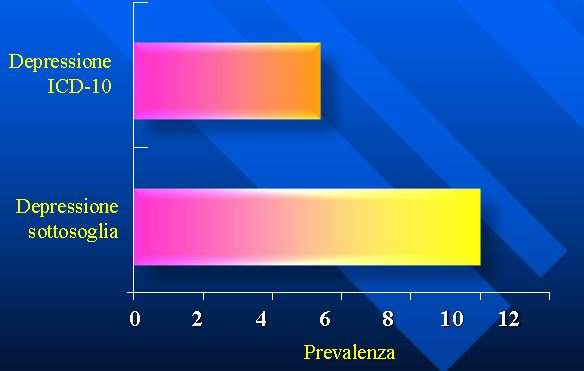
\includegraphics[width=0.8\textwidth]{42/image2.jpeg}
	\end{figure}
	
Secondo
lo studio di Bologna-Verona è stata analizzata anche la differente
prevalenza tra i casi di \textbf{depressione} classificabile secondo
ICD-10 e i casi di \textbf{depressione sottosoglia} (ovvero dove il
paziente non risponde completamente ai criteri per la depressione
maggiore, ma i sintomi risultano comunque impattanti sulla vita
dell'individuo) e si è visto che la depressione sottosoglia ha una
prevalenza maggiore.

Si è deciso quindi di affidare la comunicazione dei dati anche ai mezzi
di comunicazione di massa in modo tale da rendere consapevoli del
problema il maggior numero possibile di persone.

Qualsiasi medico deve essere consapevole della necessità di saper
costruire fin da subito un buon rapporto con il paziente con disagio
psichico al fine di migliorare l'approccio terapeutico prescindendo da
un trattamento farmacologico.

Uno studio del 1994 ha identificato la depressione come principale
perdita di giornate di lavoro all'anno. L'OMS ha inoltre detto che nel
2020 la depressione sarà ai primi due posti come perdita di giornate di
lavoro con ripercussioni anche a livello socio-economico.

Secondo ICD-10 per fare diagnosi di depressione maggiore devono essere
presenti almeno 4 sintomi di cui due tra i sintomi principali (i primi
tre) e due dei sintomi secondari per almeno due settimane:

\begin{itemize}
\item
  Umore depresso
\item
  Perdita di interesse e di piacere
\item
  Diminuita energia
\item
  Variazioni dell'appetito o del peso
\item
  Disturbi del sonno (insonnia o ipersonnia)
\item
  Rallentamento psicomotorio o agitazione
\item
  Bassa autostima (sono più frequenti le sindromi depressive negli
  adolescenti per il frantumarsi dei valori e spesso la scuola peggiora
  l'autostima e riduce la resilienza di adolescenti che già stanno
  affrontando un periodo difficile per molti punti di vista)
\item
  Senso di colpa
\item
  Difficoltà di concentrazione
\item
  Idee di morte (è difficile da trattare nel colloquio clinico ma è
  imprescindibile per capire la reale gravità del disturbo)
\end{itemize}

Il problema dell'ideazione suicidiaria è così impattante che la regione
Emilia Romagna nel 2012-2013 ha avviato due percorsi per la prevenzione
del suicidio sul territorio e in ospedale.

Tra i vari \textbf{disturbi d'ansia} i più frequenti sono:

\begin{itemize}
\item
  Fobia sociale, fobie specifiche, agorafobia
\item
  Attacchi di panico
\item
  Disturbo d'ansia generalizzato
\item
  Disturbo ossessivo-compulsivo
\item
  Disturbi somatoformi.
\end{itemize}

Focus su \textbf{attacchi di panico}: nel 1990 al Maurizio Costanzo Show
Valentina Cultrera (presidentessa della LIDAP) parlò dei suoi attacchi
di panico affermando che questo disturbo aveva molto impattato sulla sua
vita avendola anche limitata per quanto riguardava esperienze di lavoro.
Questo permise di ridurre il livello di vergogna dei pazienti con
attacco di panico e successivamente aumentarono notevolmente le
autodiagnosi.

Si pensa infatti che la differenza di incidenza (3 volte più frequente
nelle donne) sia legata al fatto che gli uomini con attacchi di panico
si sentono deboli e quindi non lo riferiscano.

Il medico dovrebbe confrontarsi con la storia, la sofferenza del
paziente e con il percorso che lo ha portato all'autodiagnosi senza
infastidirsi e offrendo la sua cultura per aiutare il paziente.

\begin{figure}[!ht]
\centering
	
\includegraphics[width=0.8\textwidth]{42/image3.jpeg}
	\end{figure}
	
In
medicina generale una buona modalità per raccogliere informazioni è
chiedere al paziente, se vuole e non lo fa stare male, di scrivere un
diario in modo da focalizzare le cose accadute.

Può essere una modalità di ascolto. Questo frammento ci fa vedere come
gli attacchi di panico possono essere frequenti in adolescenza e come
siano impattanti nella storia di un individuo tanto da ricordarlo
numerosi anni dopo.

La \textbf{depressione mascherata} è quella condizione clinica in cui un
paziente presenta diversi sintomi somatici privi di spiegazione
organica, senza lamentare esplicitamente un tono dell'umore depresso. Si
tratta di pazienti che hanno comunque un abbassamento del tono
dell'umore, ma hanno difficoltà a verbalizzarlo (alessitimia) ed
utilizzano il sintomo somatico come strumento di aggancio relazionale
con il medico.

La difficoltà a verbalizzare le emozioni può essere legata al fatto che
la persona percepisca di essere accudita solo se riferisce un sintomo
somatico.

I segni somatici con cui si manifesta la depressione mascherata sono:

\begin{itemize}
\item
  Cefalee croniche (sensazione vaga di tensione o bruciore alla testa)
\item
  Algie lombo-sacrali o cervicali
\item
  Pseudoangine (accompagnate da angoscia precordiale)
\item
  Tachicardia
\item
  Sensazione di soffocamento od oppressione
\item
  Alterazioni del ritmo del sonno
\item
  Dispnea notturna
\item
  Sensazione di astenia al risveglio
\item
  Bocca secca
\item
  Gastralgie
\item
  Nausea
\item
  Aerofagia
\item
  Stipsi/diarrea
\item
  Sintomi dolorosi addominali
\item
  Pollachiuria
\item
  Tenesmo vescicale
\item
  Algie di natura genitale che possono inficiare la funzione sessuale
\item
  Disturbi atipici dell'udito e della vista
\item
  Caduta dei capelli fino all'alopecia (caso emblematico dell'arbitro
  Collina che dopo essere stato tradito e lasciato dalla fidanzata
  divenne completamente glabro in 48 h per il forte stress).
\end{itemize}

A prima vista un sintomo somatico, come ad esempio l'algia cervicale il
lunedì mattina, potrebbe essere in realtà la drammatizzazione di un
disagio psichico legato ad una situazione in cui il paziente non si
trova a proprio agio (stress sul luogo di lavoro).

\subsection{Patologie associate a depressione dell'umore}


Esistono numerose patologie somatiche associate a depressione
dell'umore:

\begin{itemize}
\item
  Disturbi endocrini

\begin{itemize}
\item
  Ipotiroidismo: un tempo i pazienti ipotiroidei gravi finivano in
  manicomio perché obnubilati e depressi cronici
\item
  Ipertiroidismo
\item
  Diabete: spesso il paziente vive la diagnosi come una limitazione alla
  propria libertà. Inoltre la depressione è in grado di scompensare il
  diabete.
\end{itemize}

\item
  Malattie cardiovascolari

\begin{itemize}
\item
  Scompenso cardiaco congestizio: determina un'alterazione della propria
  immagine e della capacità di stare nel mondo
\item
  Infarto del miocardio
\end{itemize}

\item
  Disturbi metabolici
\item
  Malattie infettive

\begin{itemize}
\item
  Polmonite: soprattutto negli anziani può accompagnarsi a disturbi
  deliranti
\end{itemize}

\item
  Malattie polmonari

\begin{itemize}
\item
  Neoplasie polmonari
\item
  BPCO
\end{itemize}

\item
  Malattie reumatiche e immunologiche: si è visto che la depressione
  caratterizza le connettiviti soprattutto nel periodo antecedente allo
  sviluppo di malattia sotto forma di disagio psichico. Questo può
  essere importante perché se il MMG è attento ai sintomi prodromici può
  fare diagnosi precoce e trattare meglio il paziente.

\begin{itemize}
\item
  Artrite reumatoide
\item
  Polimialgia reumatica
\item
  LES
\end{itemize}

\item
  Anemie
\item
  Carenze vitaminiche
\item
  Allergopatie: si accompagnano spesso ai sintomi depressivi. Si è
  ipotizzato come fattore causale della depressione un possibile
  passaggio delle IgE attraverso la BEE.
\item
  Malattie neurologiche

\begin{itemize}
\item
  Stroke: spesso in questi pazienti la depressione è trascurata
  nonostante l'ictus lasci esiti invalidanti che impattano notevolmente
  sulla vita quotidiana del paziente (una persona che prima era autonoma
  potrebbe ritrovarsi con deficit motori e di linguaggio)
\item
  Parkinson: Citalopram (inibitore reuptake della serotonina) è il
  farmaco migliore per un paziente con Parkinson e depressione
\end{itemize}

\item
  Patologie genito-urinarie.
\end{itemize}

Si è visto inoltre che la depressione peggiora le malattie somatiche a
causa di una serie di motivi:

\begin{itemize}
\item
  Abbassa la soglia del dolore
\item
  Riduce la motivazione a curarsi
\item
  Peggiora la prognosi
\item
  Incrementa la mortalità
\item
  Incrementa la disabilità
\item
  Incrementa il carico per i caregivers
\item
  Incrementa i ricoveri ospedalieri.
\end{itemize}

Esistono numerosi farmaci che possono causare sintomi depressivi:

\begin{itemize}
\item
  Anti-ipertensivi (Reserpina è stato il primo anti-ipertensivo accusato
  di dare depressione)
\item
  Antineoplastici
\item
  Antiparkinsoniani
\item
  PPI
\item
  Corticosteroidi (causano anche ideazioni deliranti)
\item
  Anti-infiammatori
\item
  Beta-bloccanti
\item
  Contraccettivi orali
\item
  Antipsicotici
\end{itemize}

Anche alcune sostanze d'abuso possono causare ansia e/o depressione:

\begin{itemize}
\item
  Alcol o una sua sospensione
\item
  Cocaina, anfetamine e simili
\item
  Cannabis o una sua sospensione
\end{itemize}

Esistono numerose malattie in comorbidità con la depressione:

\begin{itemize}
\item
  Neurologica prevalenza 37,5\%
\item
  Coronarica prevalenza 34,6\%
\item
  Polmonare prevalenza 30,9\%
\item
  Oncologica prevalenza 30,3\%
\item
  Reumatologica prevalenza 25,3\%
\item
  Diabete prevalenza 22,7\%
\item
  Ipertensiva prevalenza 22,4\%
\end{itemize}

Roose nel 1992 ha dimostrato che soggetti depressi hanno un rischio di
mortalità nel post-infarto 3,5 volte superiore rispetto ai non depressi.

\begin{figure}[!ht]
\centering
	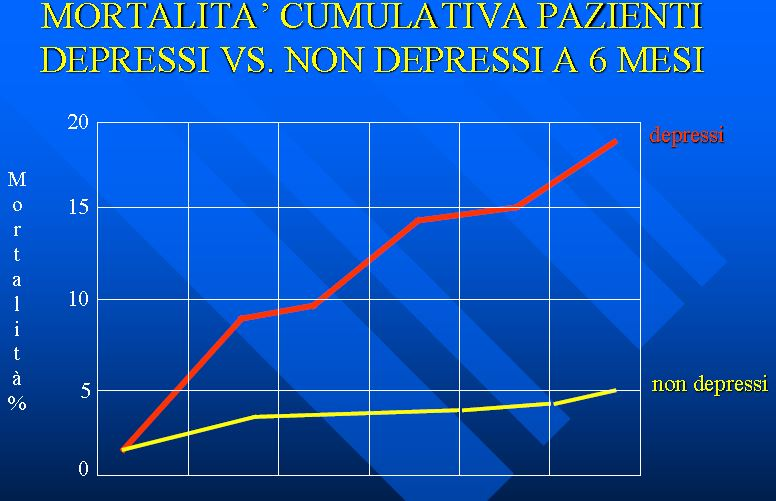
\includegraphics[width=0.8\textwidth]{42/image4.jpeg}
	\end{figure}
	
Un
disturbo depressivo insorto nel decennio precedente un evento
cardiovascolare acuto eleva di tre volte il rischio di ischemia
miocardica nel maschio.

I maschi affetti da cardiopatia ischemica presentano un rischio
depressivo più elevato rispetto ai controlli sani.

La depressione rappresenta un fattore di rischio cardiovascolare
indipendente, stabile nel tempo per diverse decadi dall'esordio
sintomatologico.

Il medico dovrebbe considerare anche la depressione quando valuta i
numerosi fattori di rischio per la cardiopatia ischemica.

Il suo impatto sulla mortalità è indipendente dalla gravità iniziale
della cardiopatia.

La depressione peggiora il decorso e la prognosi della cardiopatia
ischemica e influisce negativamente sui programmi
terapeutico-riabilitativi.

La depressione maggiore aumenta la mortalità in patologia coronarica,
aumenta la ``heart rate variability'', riduce l'aderenza alle terapie e
dà un'abnorme reattività piastrinica.

Si è visto che la depressione nei malati di tumore è trattata in modo
insufficiente: uno studio del ``Journal of Hospice and palliative
nursing'' analizzando 142 malati terminali ha concluso che il 17,6\% di
questi era affetto da depressione (ICD-10) e meno di un terzo era
trattato in modo conveniente.

Al giorno d'oggi la malattia neoplastica in molti casi è diventata
malattia cronica e perciò il paziente oncologico è spesso anche depresso
e come tale va aiutato.

Nella malattia di Alzheimer vi è un maggior rischio di disturbi
psichiatrici. Spesso la depressione ha come manifestazione clinica
l'aggressività. L'aggressività è la restituzione di una carenza di
aggrappamento, cioè il paziente vorrebbe aggrapparsi a noi, ma non ci
riesce e perciò ci aggredisce; per il paziente non siamo
sufficientemente generosi nell'accudimento.
